\documentclass{beamer}
\usetheme{metropolis}
\usepackage[estonian]{babel}
\usepackage[utf8]{inputenc}
\usepackage[normalem]{ulem}
\usepackage{csquotes}

\title{IDU1321. Ettevõtte äriarhitektuur}
\subtitle{Viies loeng}
%\date{10.09.2017}
\author{Andres Kütt}
\institute{Arhitekt}


\begin{document}

\begin{frame}
\titlepage
\end{frame}

\begin{frame}[standout]
Küsimusi loetu kohta?
\end{frame}

%\begin{frame}[standout]
%Küsimusi jagatud linkide kohta?
%\end{frame}

\begin{frame}[standout]
Küsimusi kodutöö kohta?
\end{frame}

\begin{frame}[standout]
Tagasiside!
\end{frame}

\section{Tagasiside}
\begin{frame}{Halb}

	\begin{center}
\begin{tabular}{ p{5cm} p{5cm}  }
\textbf{Mis te ütlesite} & \textbf{Mis ma teen}\\
\hline
Materjali on palju ja see on ingliskeelne & Järgmine kord ingliskeelne end tõestanud õpik. Emakeelset sisu lihtsalt ei ole\\ 
Rohkem ja väiksemaid (koduseid) praktilisi töid & Järgmine kord esitatakse projekti etapid ükshaaval\\
Ebaselge, kuidas tükkidest praktiline EA pilt moodustub & Lisan skeemi slaidi\\
\end{tabular}
\end{center}
\end{frame}


\begin{frame}{Hea}
	\begin{itemize}
		\item Õppejõud on EAga tegelenud: reaalsed näited
		\item Kodutöö võimaldab loovat lähenemist
		\item Palju taustalugemist, sellest moodustub terviklik pilt
		\item Materjalid kättesaadavad
	\end{itemize}
\end{frame}

\begin{frame}{Kus me oleme?}
	\begin{center}
		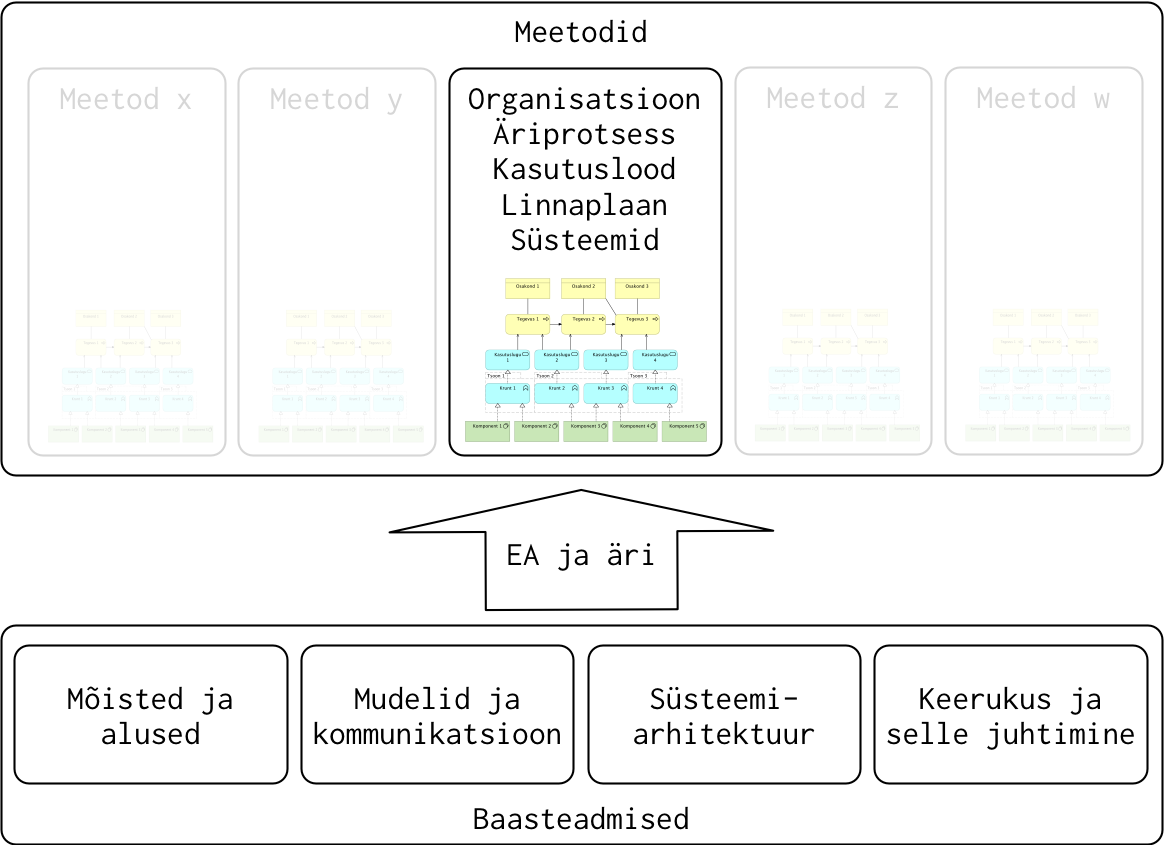
\includegraphics[width=.8\textwidth]{aine_struktuur}
	\end{center}
\end{frame}

\section{Linnaplaneerimine}
\begin{frame}{Mis see on}
	\begin{itemize}
		\item Longépé, C. (2003). The enterprise architecture IT project: the urbanisation paradigm. Elsevier
		\item Meenutage arhitekti ja ettevõttearhitekti suhet
		\item Mõelge arhitekti ja linna-arhitekti suhtele
		\item Siit idee vaadata organisatsiooni infosüsteemi kui linna
	\end{itemize}
\end{frame}

\begin{frame}[fragile]
	\begin{center}
		\LARGE{\textbf{Tegemist on pelgalt mudeliga, see metafoor lekib!}}
		\\[4cm]
		\small{Kõik mudelid on valed, mõned mudelid on kasulikud. Urbanismis on kasulikke ideid aga päris kõigi üldistustega ei saa nõus olla. Kuidas mahub siia liikluse juhtimine?}
	\end{center}
\end{frame}

\begin{frame}{Terminoloogia}
	\enquote{Linn} on jagatud osadeks:
	\begin{description}
		\item[Maakasutusplaan]\footnote{\emph{Land Usage Plan}, lühidalt LUP} on dokument, mis kirjeldab linna maa jaotust tsoonideks ning neis tsoonides toimuvat
		\item[Tsoon] koondab sarnaseid\footnote{Juhtimise, kompetentside, halduse jne. mõttes} süsteeme ning on maakasutusplaani osis
		\item[Krunt]\footnote{\emph{Plot}} on mingis tsoonis asuv süsteem või süsteemi \underline{loogiline}, konkreetset fuktsiooni täitev, osa
	\end{description}
\end{frame}

\begin{frame}[fragile]
	\begin{center}
		\LARGE{\textbf{Longépé on kirjeldanud kuus tsooni}}
		\\[4cm]
		\small{Definitsioone võib muuta, kui kommunikatsioon ei kannata ja kasulik on. Näiteks jätta ära referentsitsoon ja jagada andmetsoon turvadomeenide alusel.}
	\end{center}
\end{frame}

\begin{frame}{Tsoonid}
	\begin{description}
		\item[Ressursitsoon] Krundid, mis toetavad põhiprotsessi
		\item[Referentstsoon] Krundid, mille abil seotakse teisi süsteeme
		\item[Otsustustsoon] Krundid, mis realiseerivad juhtide otsustustoe
		\item[Andmetsoon] Krundid, mis tegelevad andmete hoidmisega
		\item[Operatsioonitsoon] Krundid, mis tegelevad otseselt põhiprotsessi realisatsiooniga
		\item[Kanalitsoon] Krundid, mis realiseerivad organisatsiooni \emph{mis iganes} suhte välismaailmaga
	\end{description}
\end{frame}

\begin{frame}{Milleks see kõik kasulik võib olla?}
	Krundist võib mõelda kui juhtimisobjektist
	
	\begin{description}
		\item[Inventuur.] Mitu kasutajaliidest ja registrit meil on?
		\item[Arendusülesanne.] Kui me tahame realiseerida muutuse äriprotsessis, siis milliseid süsteeme tuleb muuta või arendada?
		\item[Mõjuanalüüs.] Kui me muudame mõnd süsteemi, siis mis äriprotsesside mis tegevused saavad sellest mõjutatud?
		\item[Analüüsivahend.] Kui ma muudan mõnd kasutuslugu, siis milliste tehniliste piirangutega ma pean arvestama? Miks kõik tsoonid esindatud ei ole?
		\item[Projektijuhtimisvahend.] Realiseerimaks seda äriprotsessi, mis kompetentse vajavad mis tükid ma ehitama pean?
	\end{description}
\end{frame}


\begin{frame}{ICISe LUP}
	\begin{center}
		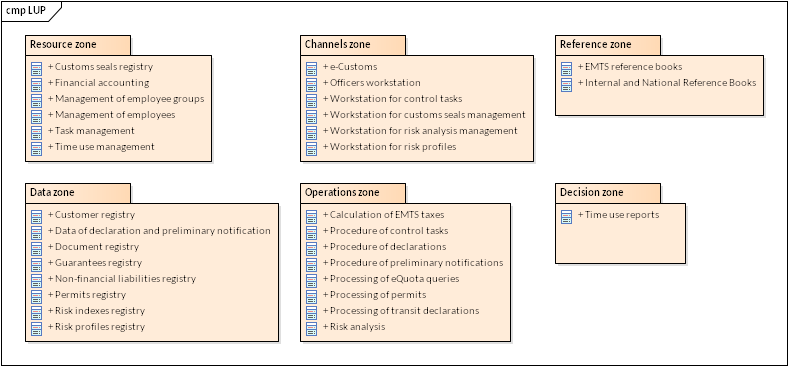
\includegraphics[width=\textwidth]{LUP.png}
	\end{center}
\end{frame}

\begin{frame}{Märkusi ICISe LUPi kohta}
	\begin{itemize}
		\item \emph{Customs seals registry} peab arvet plommide laoseisu üle, klassikaline ressursitsooni ja mitte andmetsooni krunt
		\item Kruntide abstraktsioonitase kõigub: \emph{management of employee groups} vs. \emph{financial accounting}
		\item Pange tähele x-tee liideste puudumist kanalite tsoonist
		\item Klassifikaatoreid on kaks: keskselt antavad ja kohalikud
		\item \emph{Calculation of EMTS taxes} kindlasti salvestab ka andmeid, aga see ei ole tema peamine funktsioon
	\end{itemize}
\end{frame}

\begin{frame}{LUPi koostamine}
	\begin{itemize}
		\item Lähtudes äriprotsessist
		\begin{itemize}
			\item Mis krunte mingi samm vajab? 
			\item Kas protsess läbib kõiki tsoone (st. kas me oleme kõik aspektid läbi mõelnud)?
		\end{itemize}
		\item Lähtudes tehnilistest süsteemidest
		\begin{itemize}
			\item Mis registreid/kasutajaliideseid jne me peame?
			\item Kas andmeid hoidev/porti kuulav/vms. tükk on õiges tsoonis peegeldatud?
		\end{itemize}
	\end{itemize}
	\textbf{Rusikareegel:} Mida lihtsamad on LUPi ja süsteemide kihi seosed, seda parem. Vastasel juhul kaotab krunt oma juhtimisobjekti tähenduse
\end{frame}

\begin{frame}[fragile]
	\begin{center}
		\LARGE{\textbf{Krundid ja nende jaotus tsoonidesse on kunstivorm ja mitte teadus}}
		\\[4cm]
		\small{Pea meeles LUPi koostamise eesmärki. \\Mis asju ja miks te tahate juhtida?}
	\end{center}
\end{frame}


\begin{frame}[fragile]
	\frametitle{Organisatsiooni arhitektuur}

	\begin{center}
	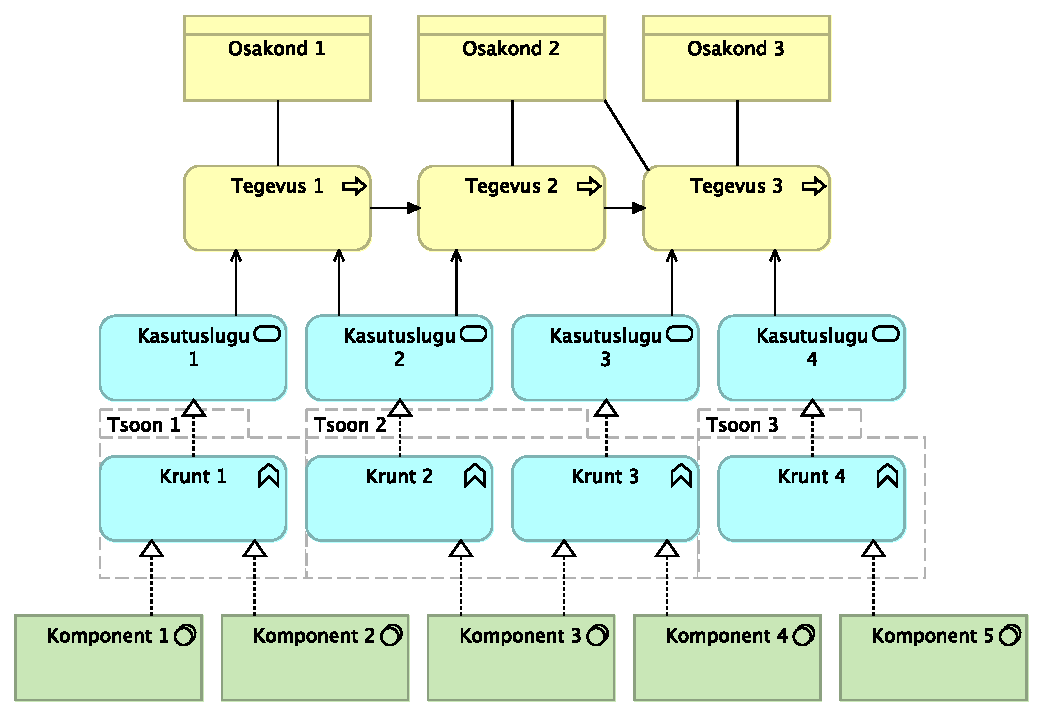
\includegraphics[width=.9\textwidth]{kihid.pdf}
	\end{center}
\end{frame}

\begin{frame}[fragile]
	\begin{center}
		\LARGE{\textbf{LUP on abstraktsioonikiht äriprotsessi ning tehnilise realisatsiooni vahel}}
		\\[4cm]
		\small{Krunte võib vaadelda \enquote{funktsionaalsete komponentidena}, nii saame rääkida ettevõtte funktsioonide staatilisest struktuurist}
	\end{center}
\end{frame}


\section{Harjutus}

\begin{frame}{Kuidas maksekorraldust realiseerida?}
Modelleerige iseteeninduses makse tegemise protsessi mõju süsteemidele
\begin{itemize}
	\item Oletame, et meil on toimiv pank ilma iseteeninduseta
	\item Loetlege kõik krundid kõigis tsoonides
	\begin{itemize}
		\item Ideaalis näidake ka seotud protsessi osiseid
	\end{itemize}
	\item Tegutsege paarides
	\begin{itemize}
		\item 18 minutit tööd mudeli kallal
		\item 12 minutit esitlete oma tööd kõrvalpaarile ja kuulate nende oma
	\end{itemize}
\end{itemize}
\end{frame}

\begin{frame}[fragile]
%	\frametitle{Organisatsiooni arhitektuur}

	\begin{center}
	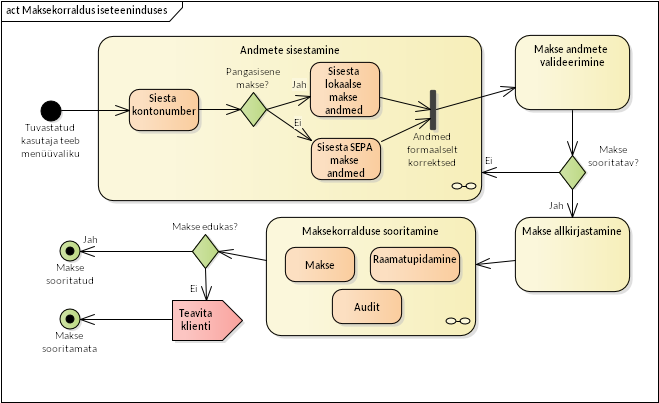
\includegraphics[width=\textwidth]{maksekasiset.png}
	\end{center}
\end{frame}


\begin{frame}{Harjutuse kokkuvõte}
	\begin{itemize}
		\item Kas kõigisse tsoonidesse tekkis midagi? 
		\item Mida ütleb saadud LUP meile organisatsiooni kohta?
		\item Mis otsuseid pidi LUPi koostamisel tegema?
	\end{itemize}
\end{frame}


\begin{frame}{Kordame}
	\begin{itemize}
		\item LUP võimaldab rääkida funktsionaalsest arhitektuurist
		\item Krunti võib vaadelda funktsionaalse juhtimisobjektina
		\item Leidub kuut liiki krunte, mida juhitakse erinevalt
	\end{itemize}
\end{frame}

\begin{frame}{Järgmine kord}
\begin{itemize}
	\item Süsteemid ja organisatsioonid
	\item Tehnilisest lahendusest äriprotsessini
	\end{itemize}
\end{frame}

%\begin{frame}{Bibliography}
%	\bibliographystyle{plainnat}
%	\bibliography{idu1321}
%\end{frame}

\begin{frame}[standout]
Küsimusi?
\end{frame}

\end{document}
